\chapter{Resultados e Discussão}

Essa seção lida com a apresentação e discussão dos resultados.
Os dados coletados são relacionados à recompensa obtida da rede neural artificial do projeto.
Com esses dados, é possível ver qual é grau de aprendizado do agente no ambiente pois a recompensa ganhada é intrinsecamente ligada ao desempenho do agente no ambiente que ele deve navegar.
Todos os ambientes usados para o treinamento da rede foram providos pela ROBOTIS, contudo, algumas alterações foram feitas no código fonte da simulação do Gazebo em ordem de usar os robô móvel simulado e a função de recompensas definida na Seção \ref{sec:r_function}.
Já os ambientes reais foram usados para avaliar se as redes propostas são capazes de fazer a atividade proposta pelo trabalho.

\section{Resultados de Simulação}

Um robô móvel com uma rede DPPG e SAC foram treinados em ordem de fazer os experimentos nos ambientes apresentados na Figura \ref{fig:environments}, onde o objetivo do agente é chegar ao alvo.
O teste inicial usou o primeiro ambiente definido.
É mostrado na Figura \ref{fig:sim_env1} uma sequência de quadros do robô até o alvo.
Nós podemos observar como o robô começou em uma posição inicial distante do alvo, para ambas as redes, navegando em ordem de chegar até o seu objetivo.

\vspace{0.25cm}
\begin{figure}[H]
\caption{Imagens sequência no primeiro ambiente simulado do experimento}
    \begin{center}
    \begin{subfigure}[b]{0.60\textwidth}
        \begin{subfigure}[b]{0.24\textwidth}
            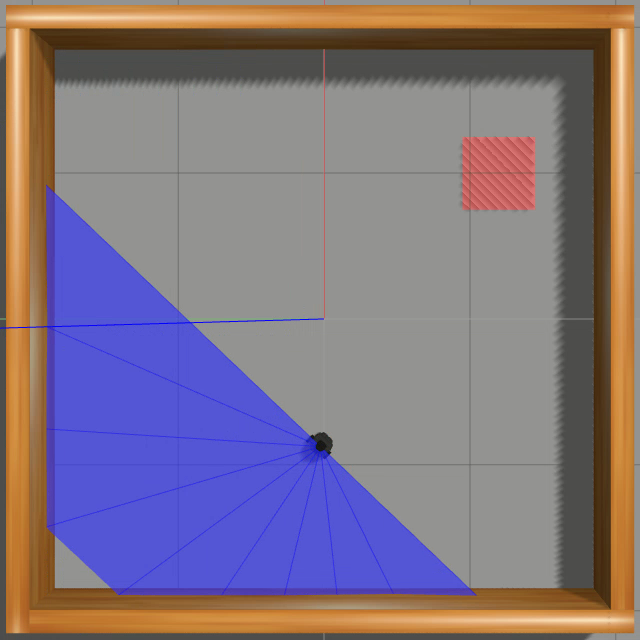
\includegraphics[width=\textwidth]{imagens/simulated_envs/sim_env1_ddpg/1.png}
        \end{subfigure}
        \hfill
        \begin{subfigure}[b]{0.24\textwidth}
            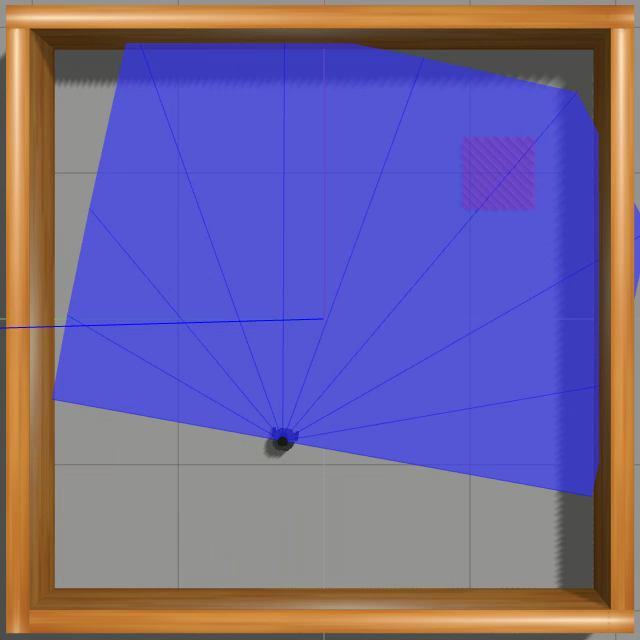
\includegraphics[width=\textwidth]{imagens/simulated_envs/sim_env1_ddpg/2.png}
        \end{subfigure}
        \hfill
        \begin{subfigure}[b]{0.24\textwidth}
            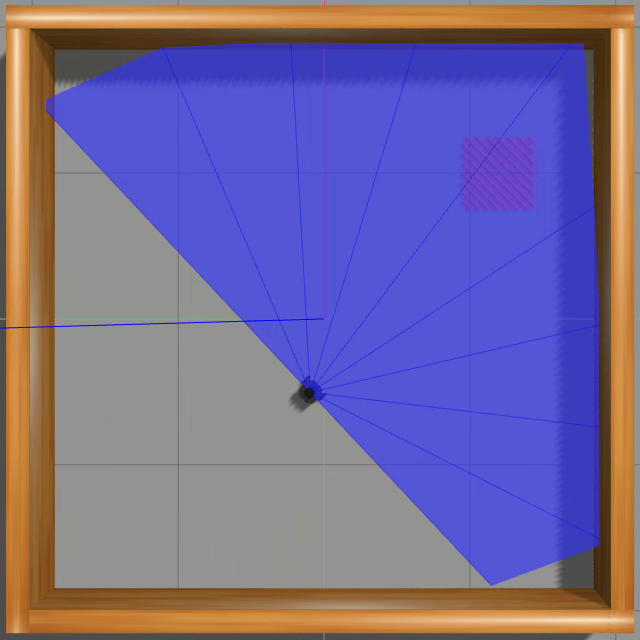
\includegraphics[width=\textwidth]{imagens/simulated_envs/sim_env1_ddpg/3.png}
        \end{subfigure}
        \hfill
        \begin{subfigure}[b]{0.24\textwidth}
            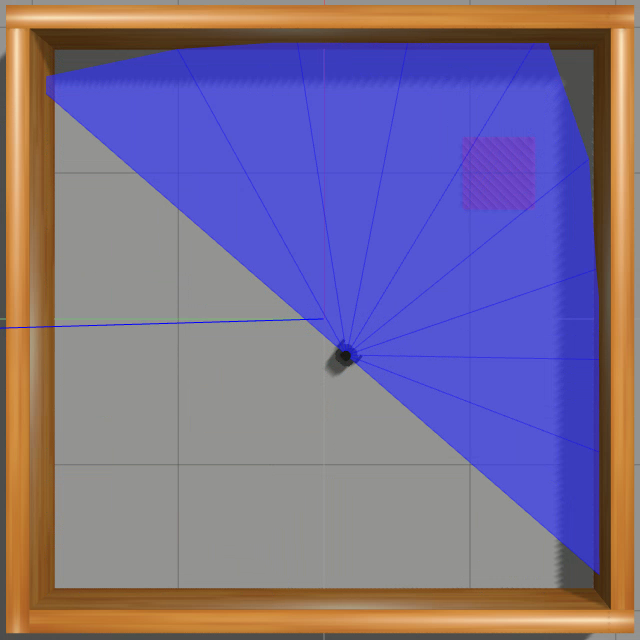
\includegraphics[width=\textwidth]{imagens/simulated_envs/sim_env1_ddpg/4.png}
        \end{subfigure}
        
        \begin{subfigure}[b]{0.24\textwidth}
            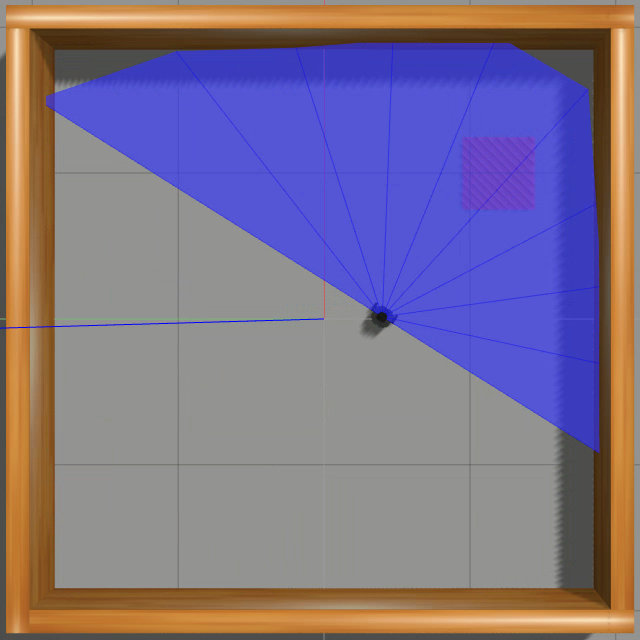
\includegraphics[width=\textwidth]{imagens/simulated_envs/sim_env1_ddpg/5.png}
        \end{subfigure}
        \hfill
        \begin{subfigure}[b]{0.24\textwidth}
            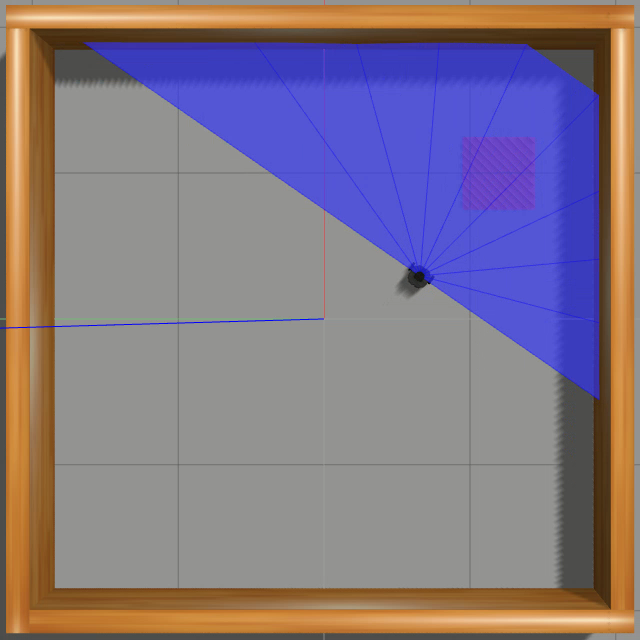
\includegraphics[width=\textwidth]{imagens/simulated_envs/sim_env1_ddpg/6.png}
        \end{subfigure}
        \hfill
        \begin{subfigure}[b]{0.24\textwidth}
            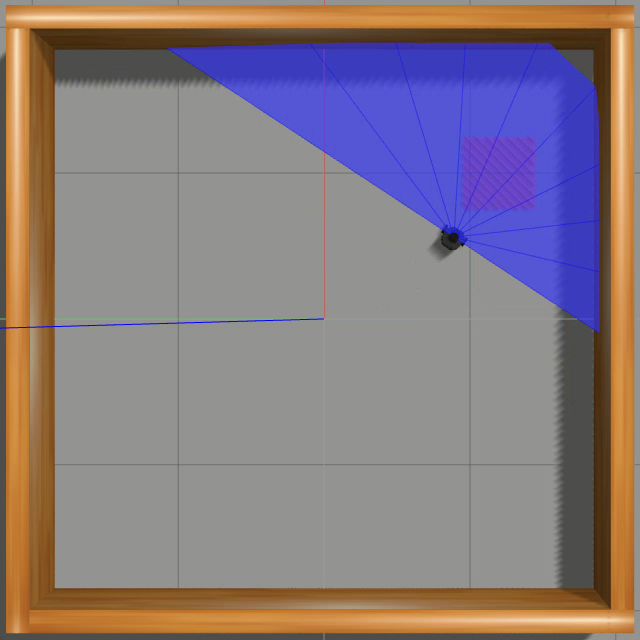
\includegraphics[width=\textwidth]{imagens/simulated_envs/sim_env1_ddpg/7.png}
        \end{subfigure}
        \hfill
        \begin{subfigure}[b]{0.24\textwidth}
            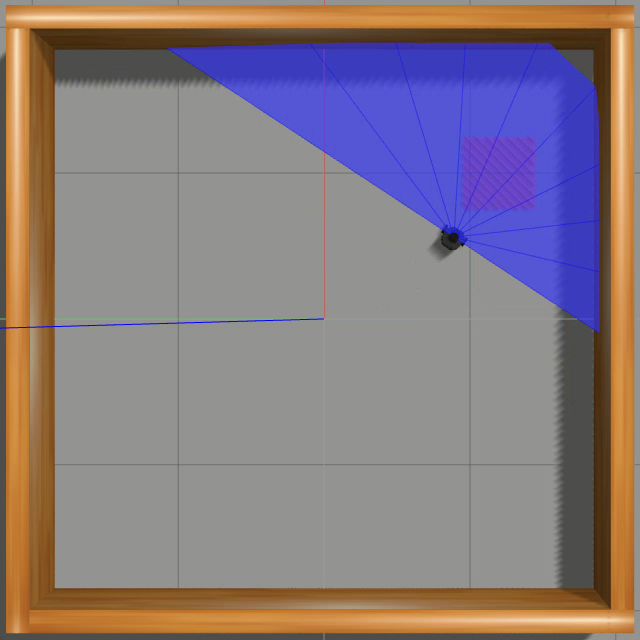
\includegraphics[width=\textwidth]{imagens/simulated_envs/sim_env1_ddpg/7.png}
        \end{subfigure}
        \caption{Rede DDPG}
        \label{subfig:simulated_env1_ddpg}
    \end{subfigure}
     %add desired spacing between images, e. g. ~, \quad, \qquad, \hfill etc. 
      %(or a blank line to force the subfigure onto a new line)
      
    \begin{subfigure}[b]{0.60\textwidth}
        \begin{subfigure}[b]{0.24\textwidth}
            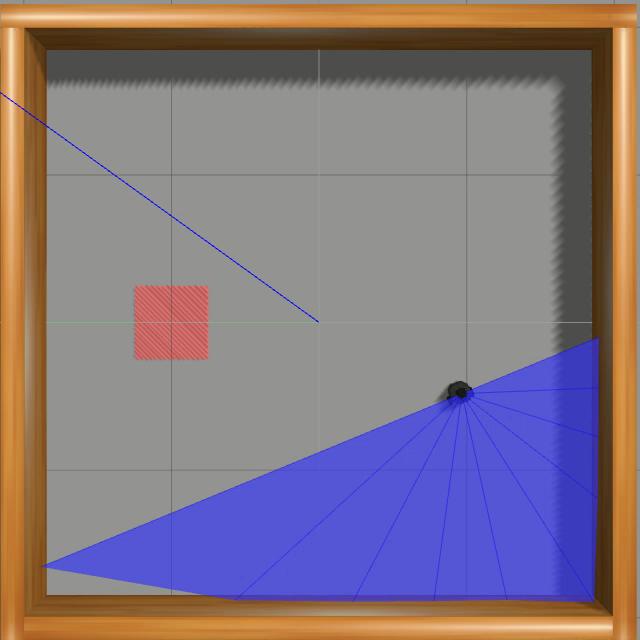
\includegraphics[width=\textwidth]{imagens/simulated_envs/sim_env1_sac/1.png}
        \end{subfigure}
        \hfill
        \begin{subfigure}[b]{0.24\textwidth}
            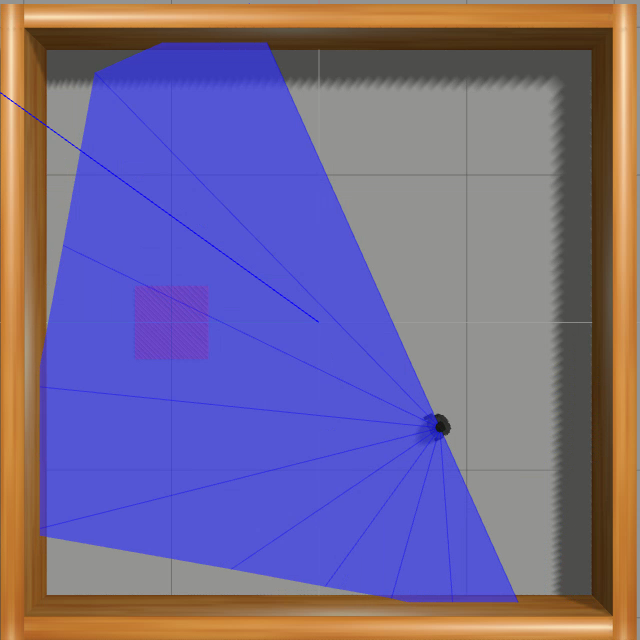
\includegraphics[width=\textwidth]{imagens/simulated_envs/sim_env1_sac/2.png}
        \end{subfigure}
        \hfill
        \begin{subfigure}[b]{0.24\textwidth}
            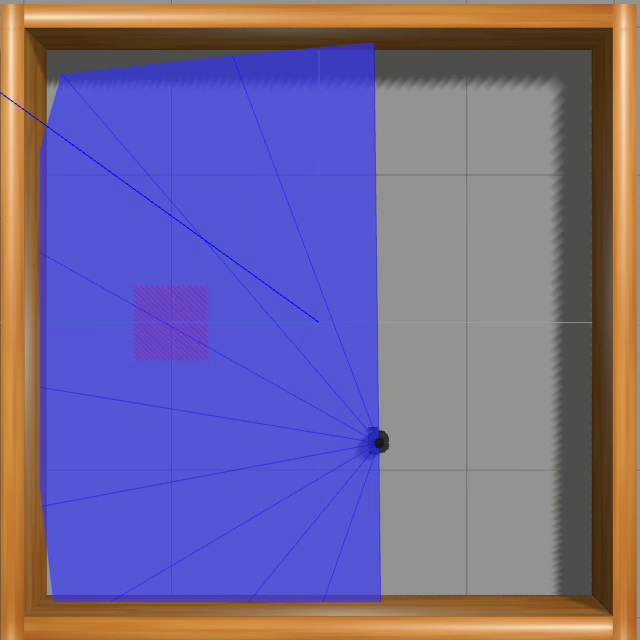
\includegraphics[width=\textwidth]{imagens/simulated_envs/sim_env1_sac/3.png}
        \end{subfigure}
        \hfill
        \begin{subfigure}[b]{0.24\textwidth}
            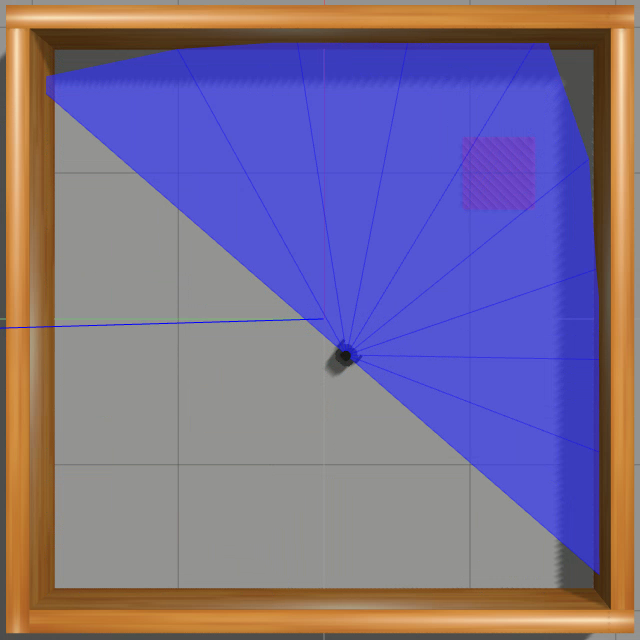
\includegraphics[width=\textwidth]{imagens/simulated_envs/sim_env1_ddpg/4.png}
        \end{subfigure}
        
        \begin{subfigure}[b]{0.24\textwidth}
            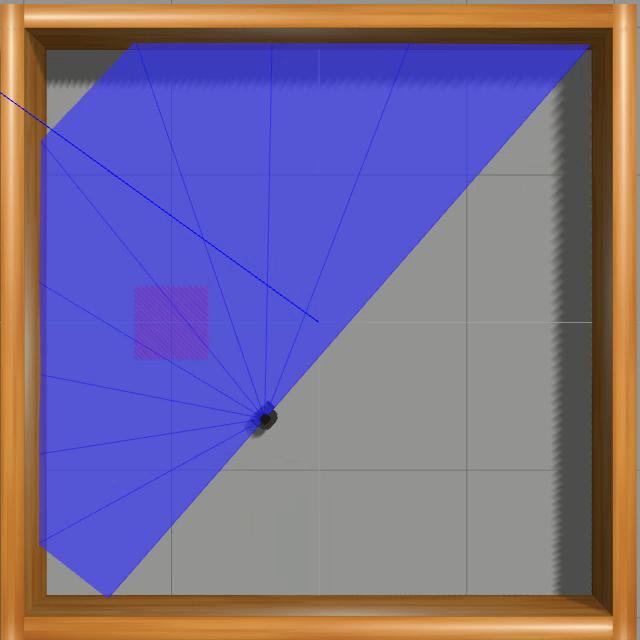
\includegraphics[width=\textwidth]{imagens/simulated_envs/sim_env1_sac/5.png}
        \end{subfigure}
        \hfill
        \begin{subfigure}[b]{0.24\textwidth}
            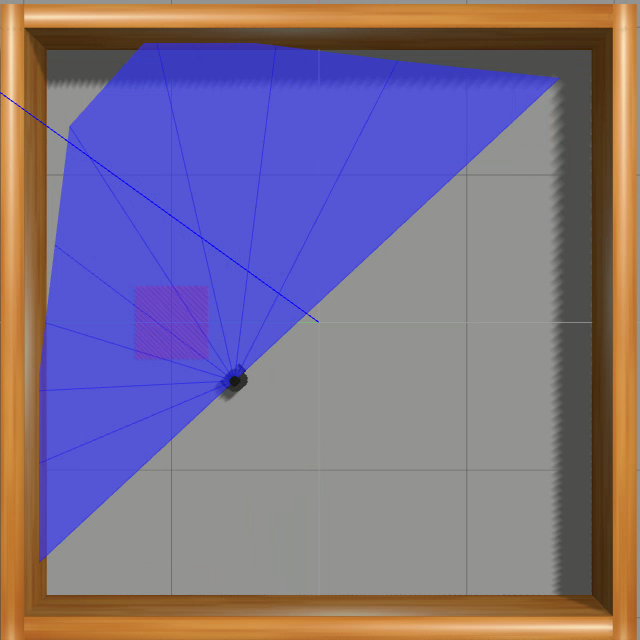
\includegraphics[width=\textwidth]{imagens/simulated_envs/sim_env1_sac/6.png}
        \end{subfigure}
        \hfill
        \begin{subfigure}[b]{0.24\textwidth}
            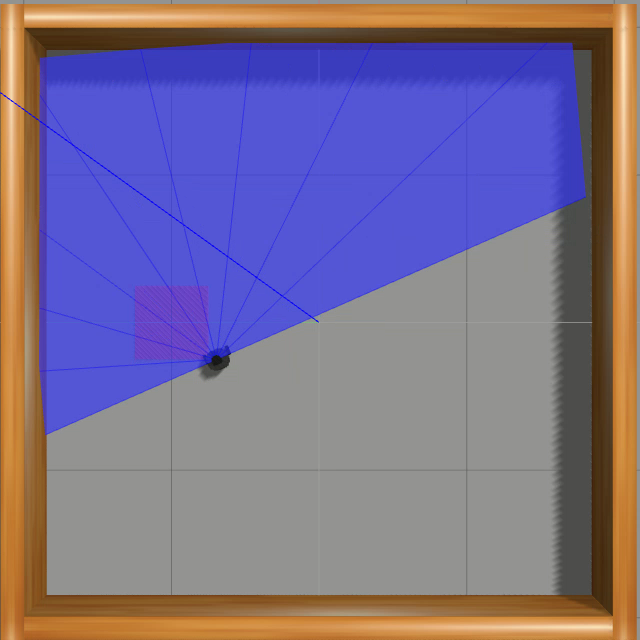
\includegraphics[width=\textwidth]{imagens/simulated_envs/sim_env1_sac/7.png}
        \end{subfigure}
        \hfill
        \begin{subfigure}[b]{0.24\textwidth}
            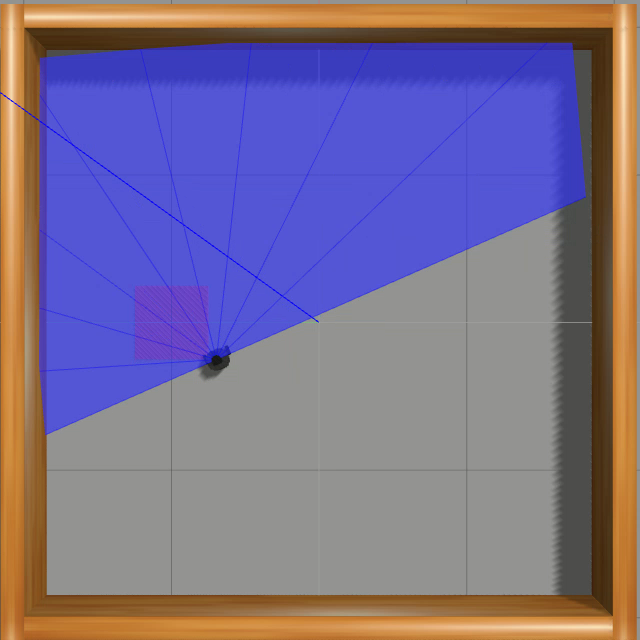
\includegraphics[width=\textwidth]{imagens/simulated_envs/sim_env1_sac/7.png}
        \end{subfigure}
        \caption{Rede SAC}
        \label{subfig:simulated_env1_sac}
    \end{subfigure}
    \label{fig:sim_env1}
    \end{center}
\small{Fonte: Autor}
\end{figure}

Os resultados do treinamento da função de recompensa do primeiro ambiente, para ambas redes, são mostrados na Figura \ref{fig:stage_1}. Nos primeiros episódios de treinamento das redes é notada uma recompensa negativa.
Isso acontece pois o algoritmo começou e ainda está em aprendizado.
Essa recompensa por episódio significa que o robô está tentando maximizar a recompensa da tarefa.
Na rede DDPG, na Figura \ref{subfig:ddpg_stage_1}, é possível ver que ela levou mais episódio para adquirir a mesma recompensa por episódio em comparação com a rede SAC, na Figura \ref{subfig:sac_stage_1}, para o mesmo episódio de treinamento.

\vspace{0.25cm}
\begin{figure}[H]
\caption{Recompensas do primeiro ambiente simulado}
    \begin{center}
    \begin{subfigure}[b]{0.48\textwidth}
        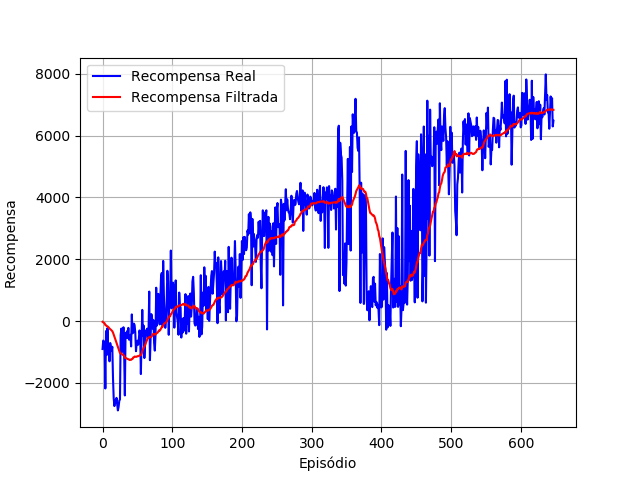
\includegraphics[width=\textwidth]{imagens/simulated_envs/ddpg_stage_1.png}
        \caption{Rede DDPG}
        \label{subfig:ddpg_stage_1}
    \end{subfigure}
    ~
    \begin{subfigure}[b]{0.48\textwidth}
        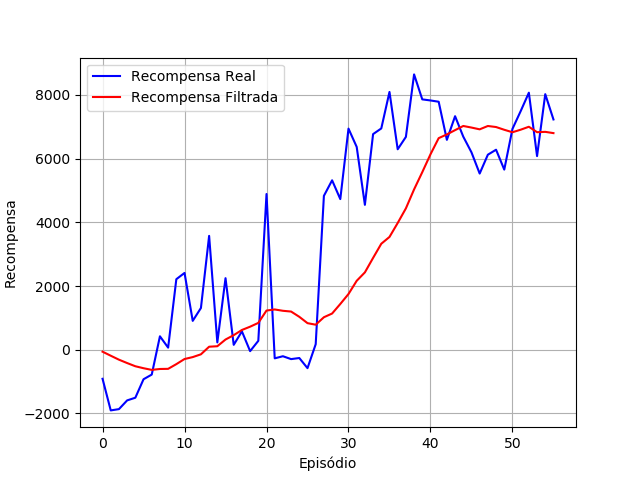
\includegraphics[width=\textwidth]{imagens/simulated_envs/sac_stage_1.png}
        \caption{Rede SAC}
        \label{subfig:sac_stage_1}
    \end{subfigure}
    \end{center}
    \label{fig:stage_1}
\small{Fonte: Autor}
\end{figure}

Na Figura \ref{fig:stage_1} o eixo $x$ representa os episódios passados na simulação, um episódio é definido quando o robô móvel chega até o alvo no mapa ou colide com algum obstáculo.
O eixo $y$, na Figura \ref{fig:stage_1}, representa o valor total da recompensa que o agente recebeu no episódio.
A recompensa, com a cor azul, tem uma grande variância. Foi decidido usar um filtro de médio móvel para melhorar a visualização dos resultados obtidos.

Depois do robô móvel ter sido treinado no primeiro ambiente, o experimento foi feito no segundo ambiente de simulação.
É mostrado na Figura \ref{fig:sim_env2} uma sequência de ações feitas pelo Turtlebot de uma posição inicial até que ele possa chegar ao alvo depois dos episódios de treinamento.

\vspace{0.25cm}
\begin{figure}[H]
\caption{Imagens sequência no segundo ambiente simulado do experimento}
    \begin{center}
    \begin{subfigure}[b]{0.60\textwidth}
        \begin{subfigure}[b]{0.24\textwidth}
            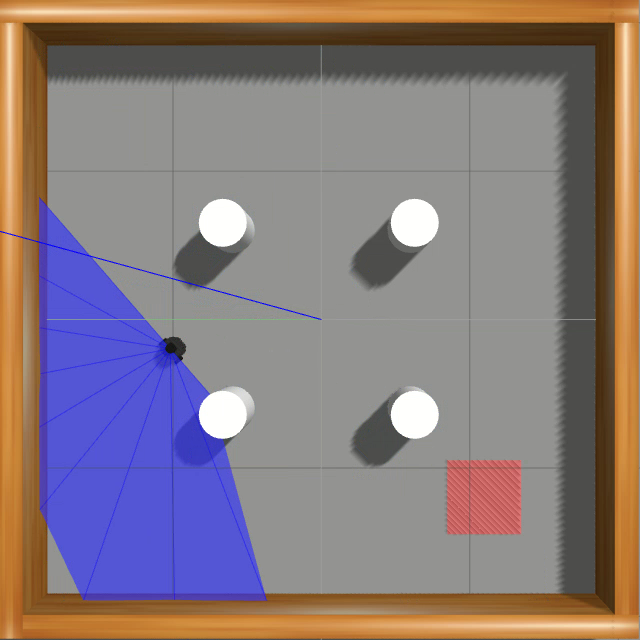
\includegraphics[width=\textwidth]{imagens/simulated_envs/sim_env2_ddpg/1.png}
        \end{subfigure}
        \hfill
        \begin{subfigure}[b]{0.24\textwidth}
            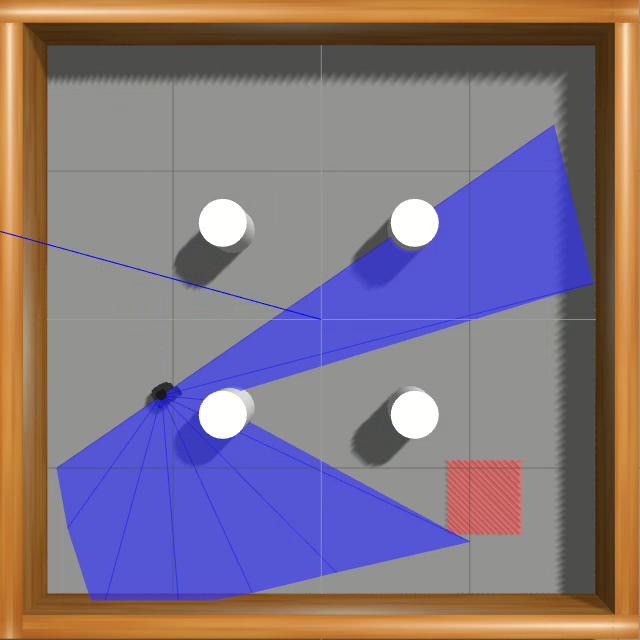
\includegraphics[width=\textwidth]{imagens/simulated_envs/sim_env2_ddpg/2.png}
        \end{subfigure}
        \hfill
        \begin{subfigure}[b]{0.24\textwidth}
            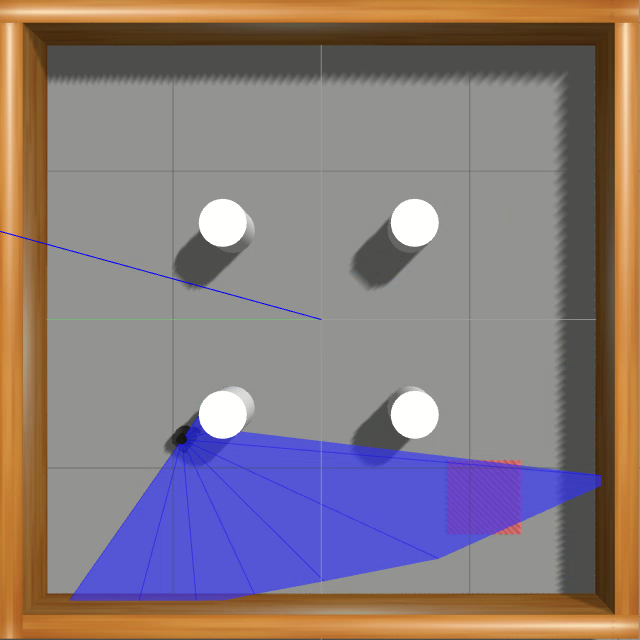
\includegraphics[width=\textwidth]{imagens/simulated_envs/sim_env2_ddpg/3.png}
        \end{subfigure}
        \hfill
        \begin{subfigure}[b]{0.24\textwidth}
            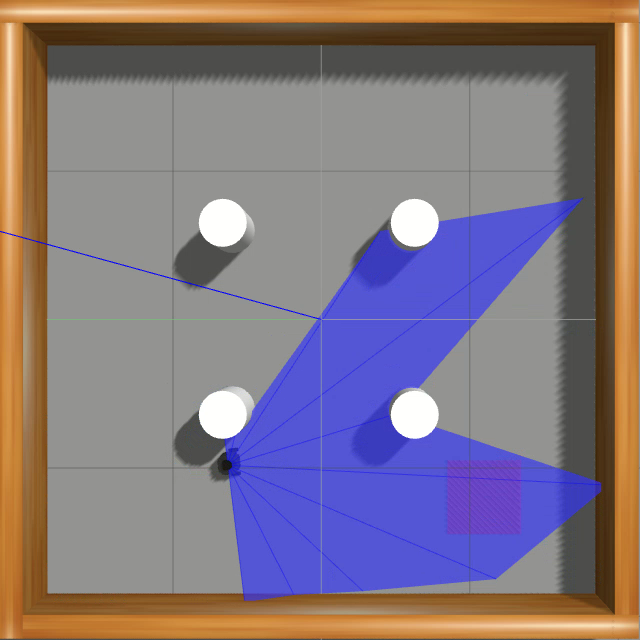
\includegraphics[width=\textwidth]{imagens/simulated_envs/sim_env2_ddpg/4.png}
        \end{subfigure}
        
        \begin{subfigure}[b]{0.24\textwidth}
            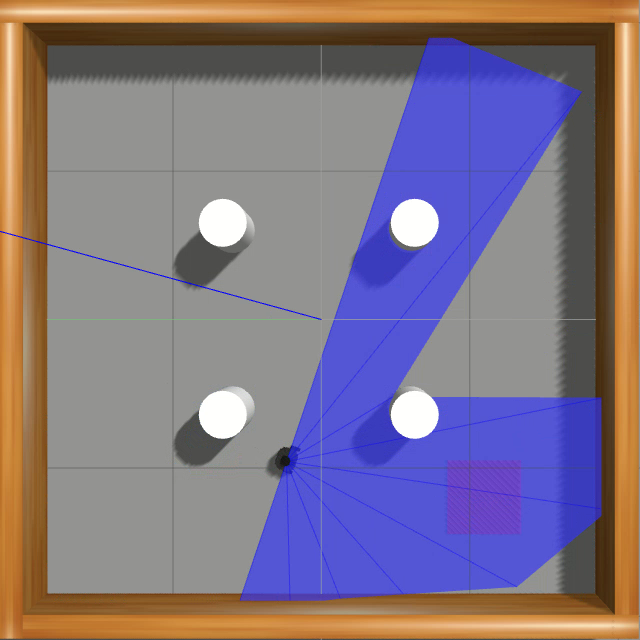
\includegraphics[width=\textwidth]{imagens/simulated_envs/sim_env2_ddpg/5.png}
        \end{subfigure}
        \hfill
        \begin{subfigure}[b]{0.24\textwidth}
            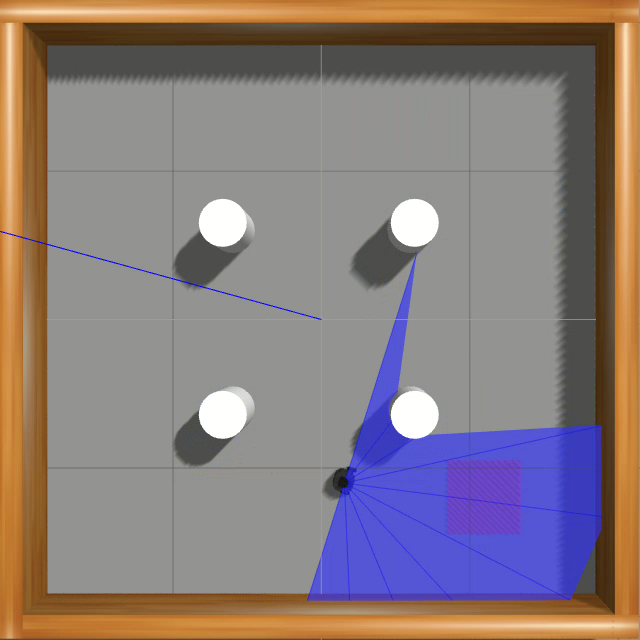
\includegraphics[width=\textwidth]{imagens/simulated_envs/sim_env2_ddpg/6.png}
        \end{subfigure}
        \hfill
        \begin{subfigure}[b]{0.24\textwidth}
            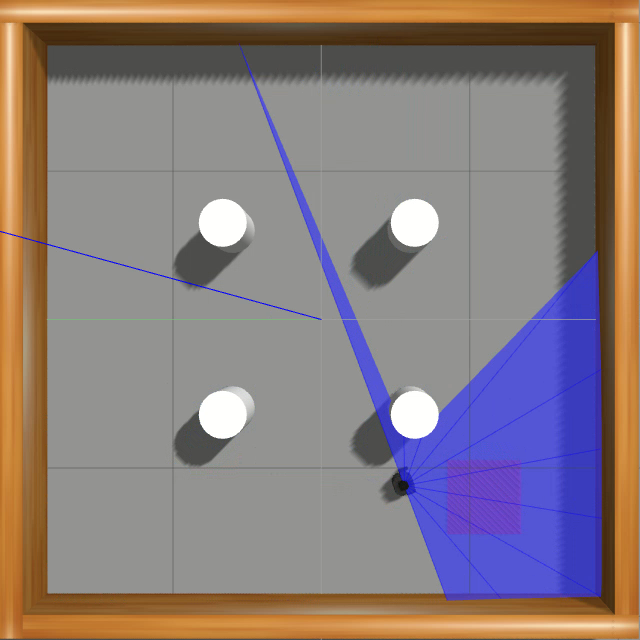
\includegraphics[width=\textwidth]{imagens/simulated_envs/sim_env2_ddpg/7.png}
        \end{subfigure}
        \hfill
        \begin{subfigure}[b]{0.24\textwidth}
            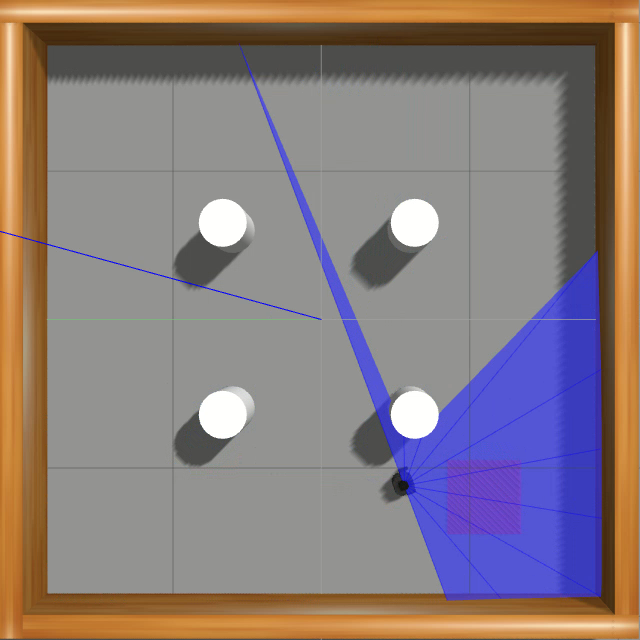
\includegraphics[width=\textwidth]{imagens/simulated_envs/sim_env2_ddpg/7.png}
        \end{subfigure}
        \caption{Rede DDPG}
        \label{subfig:simulated_env2_ddpg}
    \end{subfigure}
     %add desired spacing between images, e. g. ~, \quad, \qquad, \hfill etc. 
      %(or a blank line to force the subfigure onto a new line)
      
    \begin{subfigure}[b]{0.60\textwidth}
        \begin{subfigure}[b]{0.24\textwidth}
            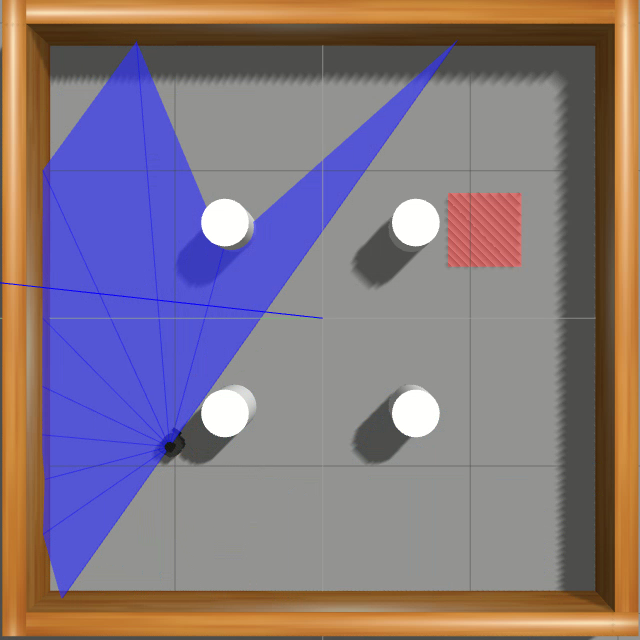
\includegraphics[width=\textwidth]{imagens/simulated_envs/sim_env2_sac/1.png}
        \end{subfigure}
        \hfill
        \begin{subfigure}[b]{0.24\textwidth}
            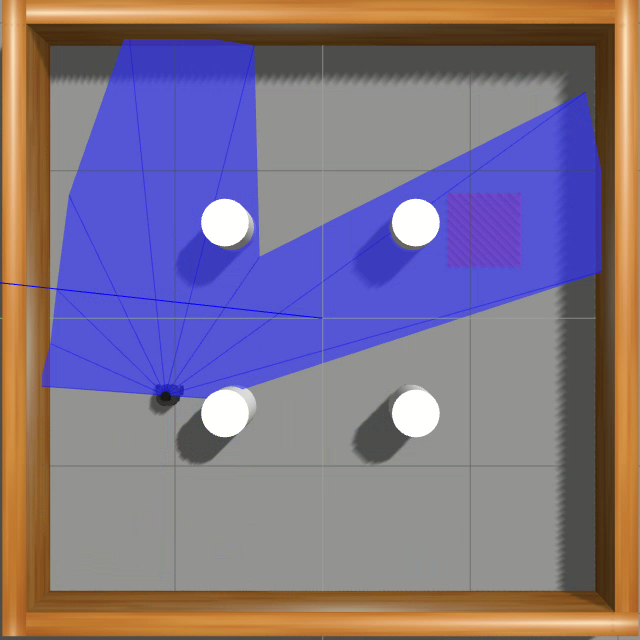
\includegraphics[width=\textwidth]{imagens/simulated_envs/sim_env2_sac/2.png}
        \end{subfigure}
        \hfill
        \begin{subfigure}[b]{0.24\textwidth}
            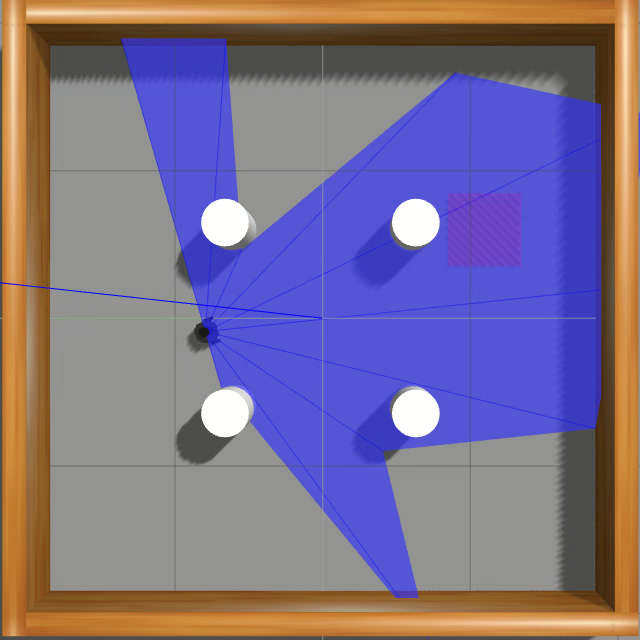
\includegraphics[width=\textwidth]{imagens/simulated_envs/sim_env2_sac/3.png}
        \end{subfigure}
        \hfill
        \begin{subfigure}[b]{0.24\textwidth}
            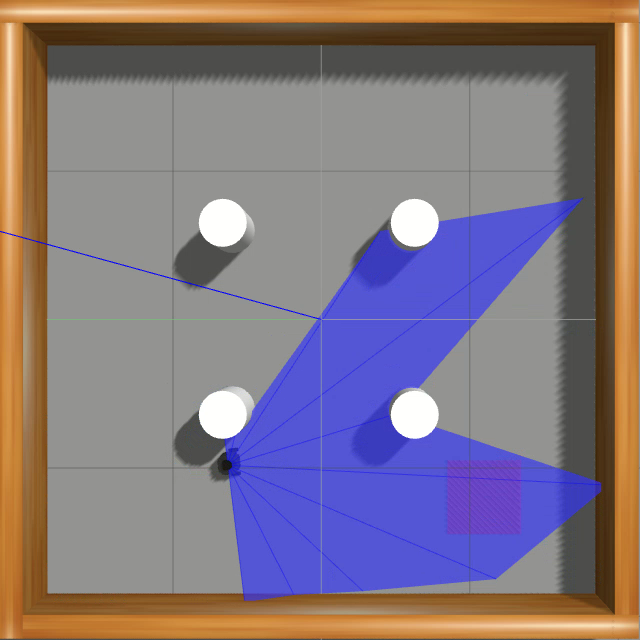
\includegraphics[width=\textwidth]{imagens/simulated_envs/sim_env2_ddpg/4.png}
        \end{subfigure}
        
        \begin{subfigure}[b]{0.24\textwidth}
            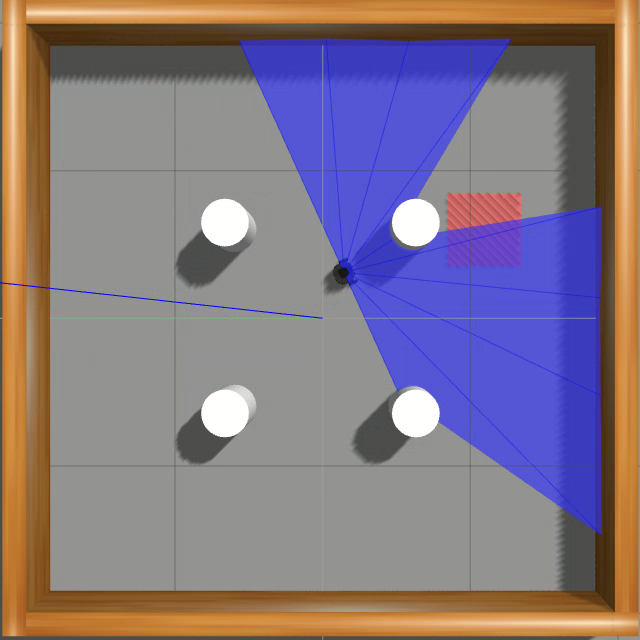
\includegraphics[width=\textwidth]{imagens/simulated_envs/sim_env2_sac/5.png}
        \end{subfigure}
        \hfill
        \begin{subfigure}[b]{0.24\textwidth}
            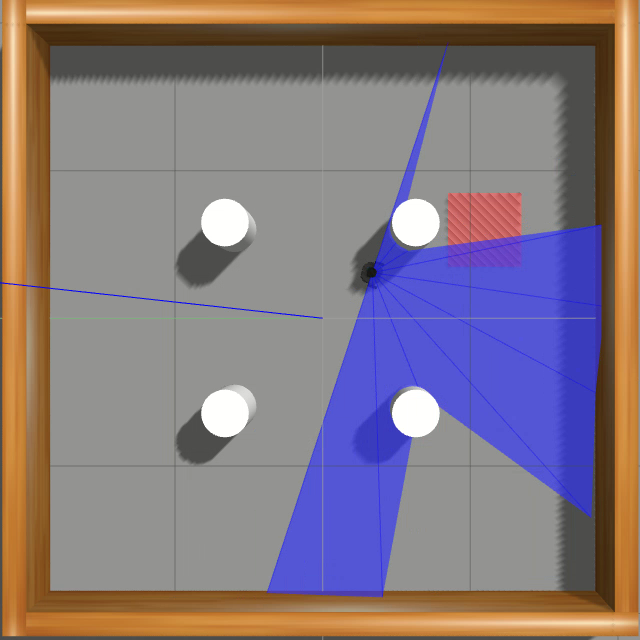
\includegraphics[width=\textwidth]{imagens/simulated_envs/sim_env2_sac/6.png}
        \end{subfigure}
        \hfill
        \begin{subfigure}[b]{0.24\textwidth}
            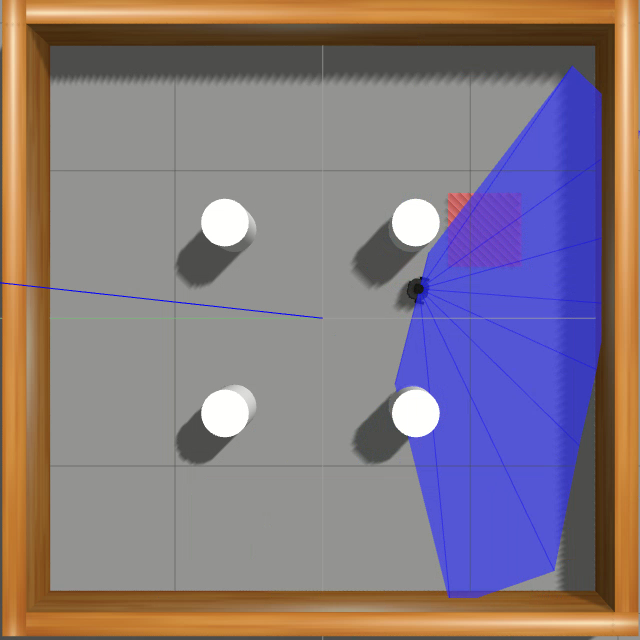
\includegraphics[width=\textwidth]{imagens/simulated_envs/sim_env2_sac/7.png}
        \end{subfigure}
        \hfill
        \begin{subfigure}[b]{0.24\textwidth}
            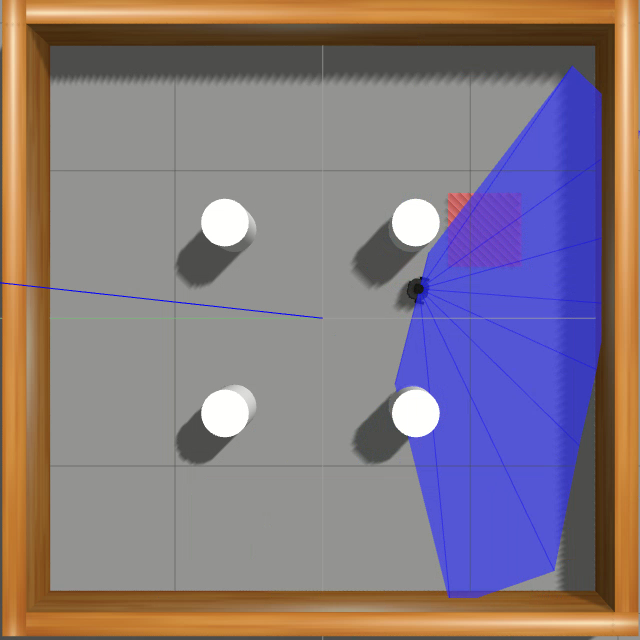
\includegraphics[width=\textwidth]{imagens/simulated_envs/sim_env2_sac/7.png}
        \end{subfigure}
        \caption{Rede SAC}
        \label{subfig:simulated_env2_sac}
    \end{subfigure}
    \label{fig:sim_env2}
    \end{center}
\small{Fonte: Autor}
\end{figure}

Os resultados da função de recompensa para o processo de treinamento do segundo ambiente de simulação são mostrados na Figura \ref{fig:stage_2}. 
Comparando esses resultados com último ambiente de simulação, é possível observar que é preciso mais episódios para que então o robô possa apresentar melhores resultados.
É notado que com um ambiente mais complexo, existe a possibilidade que um agente possa tomar um tempo mais longo para chegar a ter um bom desempenho.
E quando é posto em comparação a rede DDPG e SAC da Figura \ref{subfig:ddpg_stage_2} e Figura \ref{subfig:sac_stage_2}, respectivamente para o segundo ambiente de simulação, é possível ver que a rede SAC levou um número menor de episódios para obter a mesma recompensa por episódio da rede DDPG. 

\vspace{0.25cm}
\begin{figure}[H]
\caption{Recompensas do segundo ambiente simulado}
    \begin{center}
    \begin{subfigure}[b]{0.48\textwidth}
        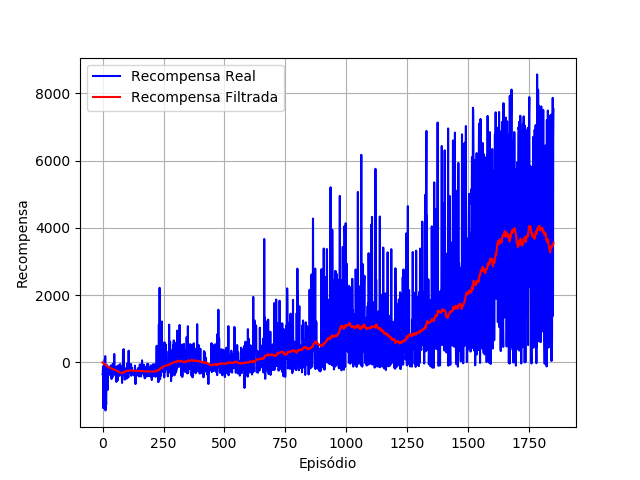
\includegraphics[width=\textwidth]{imagens/simulated_envs/ddpg_stage_2.png}
        \caption{Rede DDPG}
        \label{subfig:ddpg_stage_2}
    \end{subfigure}
    ~
    \begin{subfigure}[b]{0.48\textwidth}
        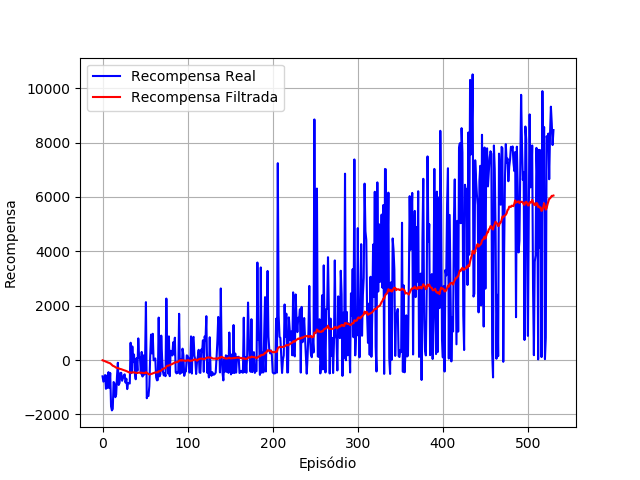
\includegraphics[width=\textwidth]{imagens/simulated_envs/sac_stage_2.png}
        \caption{Rede SAC}
        \label{subfig:sac_stage_2}
    \end{subfigure}
    \end{center}
    \label{fig:stage_2}
\small{Fonte: Autor}
\end{figure}

Para o teste final e sequência de ações feitas pelo Turtlebot para chegar até o alvo depois do processo de treinamento foi usado o terceiro ambiente simulado.
Uma sequência das ações feitas pelo robô para chegar ao alvo depois dos episódios de treinamento são mostradas na Figura \ref{fig:sim_env3}.

\vspace{0.25cm}
\begin{figure}[H]
\caption{Imagens sequência no terceiro ambiente simulado do experimento}
    \begin{center}
    \begin{subfigure}[b]{0.60\textwidth}
        \begin{subfigure}[b]{0.24\textwidth}
            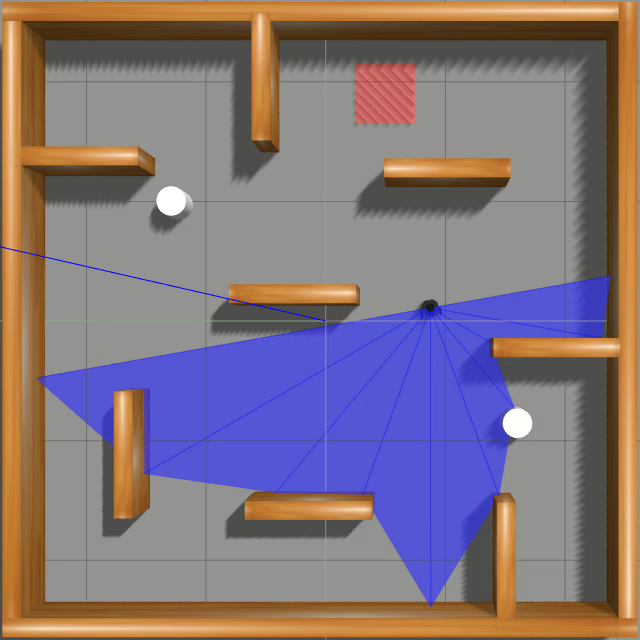
\includegraphics[width=\textwidth]{imagens/simulated_envs/sim_env3_ddpg/1.png}
        \end{subfigure}
        \hfill
        \begin{subfigure}[b]{0.24\textwidth}
            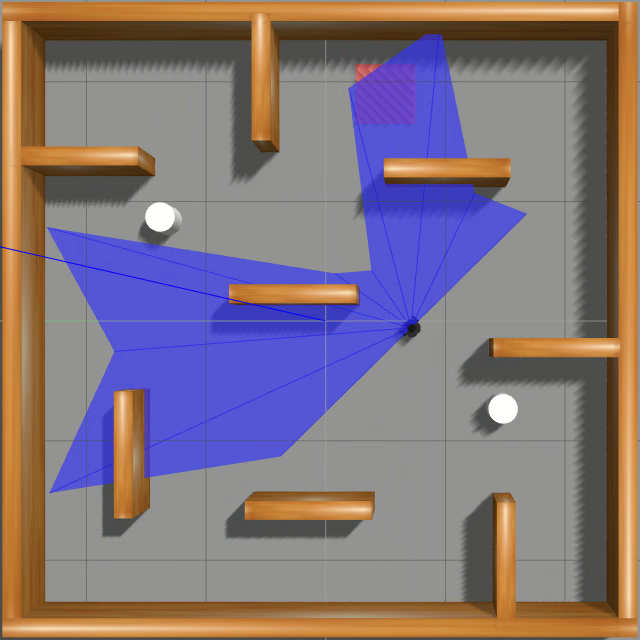
\includegraphics[width=\textwidth]{imagens/simulated_envs/sim_env3_ddpg/2.png}
        \end{subfigure}
        \hfill
        \begin{subfigure}[b]{0.24\textwidth}
            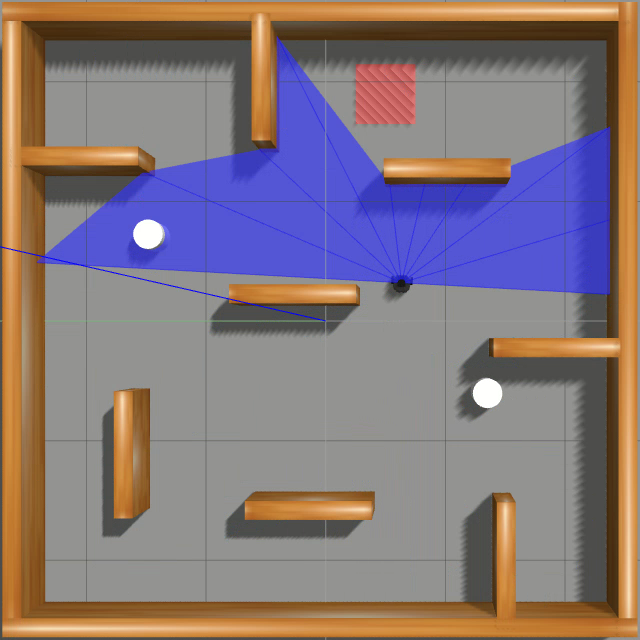
\includegraphics[width=\textwidth]{imagens/simulated_envs/sim_env3_ddpg/3.png}
        \end{subfigure}
        \hfill
        \begin{subfigure}[b]{0.24\textwidth}
            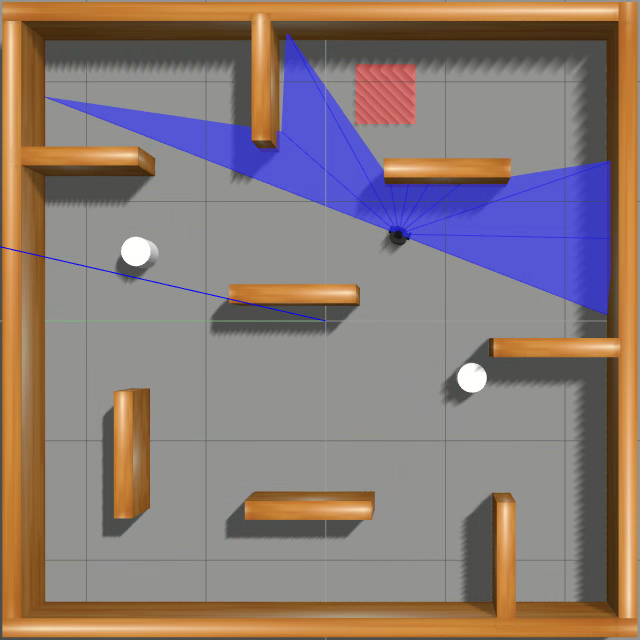
\includegraphics[width=\textwidth]{imagens/simulated_envs/sim_env3_ddpg/4.png}
        \end{subfigure}
        
        \begin{subfigure}[b]{0.24\textwidth}
            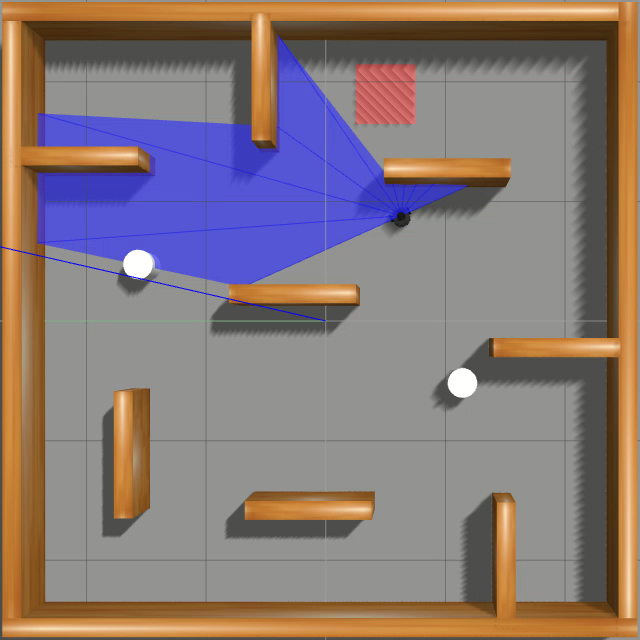
\includegraphics[width=\textwidth]{imagens/simulated_envs/sim_env3_ddpg/5.png}
        \end{subfigure}
        \hfill
        \begin{subfigure}[b]{0.24\textwidth}
            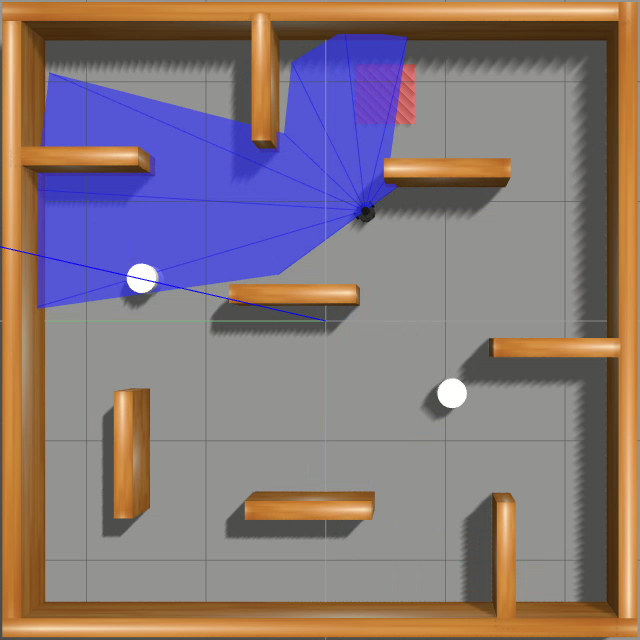
\includegraphics[width=\textwidth]{imagens/simulated_envs/sim_env3_ddpg/6.png}
        \end{subfigure}
        \hfill
        \begin{subfigure}[b]{0.24\textwidth}
            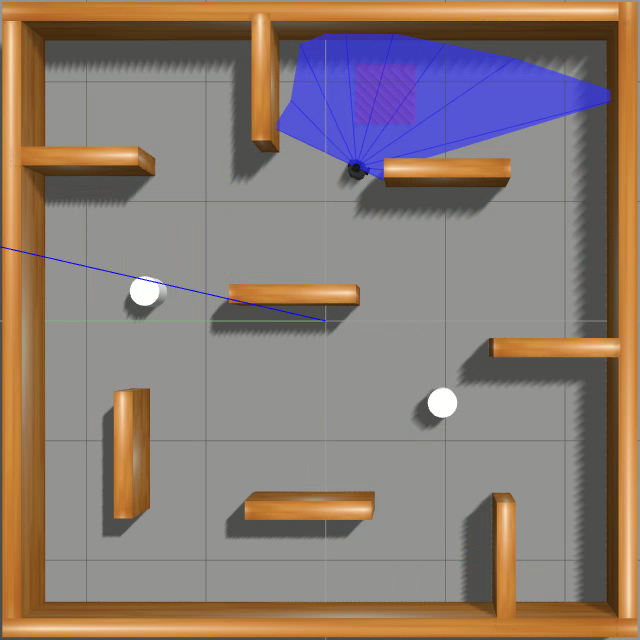
\includegraphics[width=\textwidth]{imagens/simulated_envs/sim_env3_ddpg/7.png}
        \end{subfigure}
        \hfill
        \begin{subfigure}[b]{0.24\textwidth}
            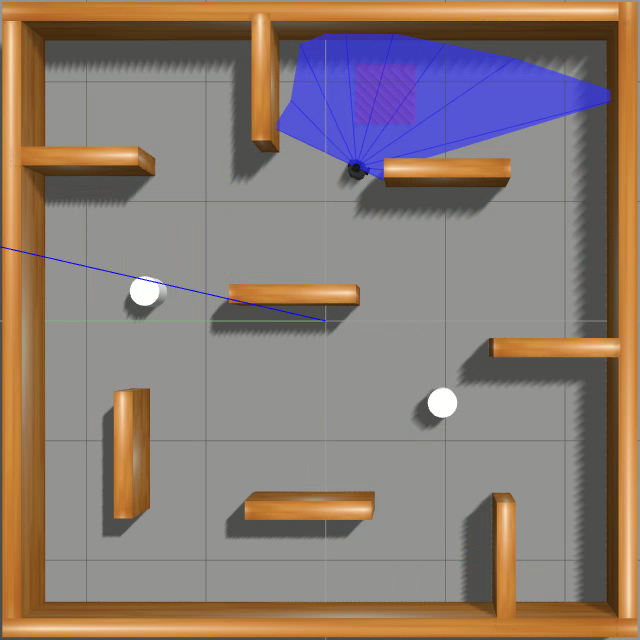
\includegraphics[width=\textwidth]{imagens/simulated_envs/sim_env3_ddpg/7.png}
        \end{subfigure}
        \caption{Rede DDPG}
        \label{subfig:simulated_env3_ddpg}
    \end{subfigure}
     %add desired spacing between images, e. g. ~, \quad, \qquad, \hfill etc. 
      %(or a blank line to force the subfigure onto a new line)
      
    \begin{subfigure}[b]{0.60\textwidth}
        \begin{subfigure}[b]{0.24\textwidth}
            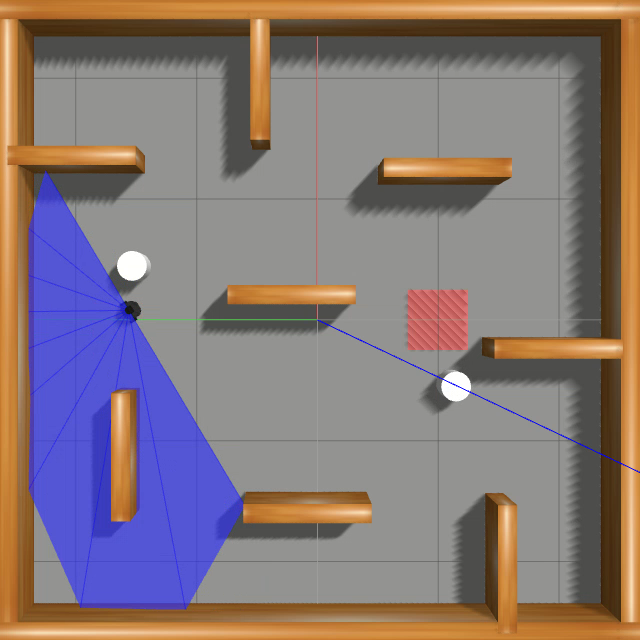
\includegraphics[width=\textwidth]{imagens/simulated_envs/sim_env3_sac/1.png}
        \end{subfigure}
        \hfill
        \begin{subfigure}[b]{0.24\textwidth}
            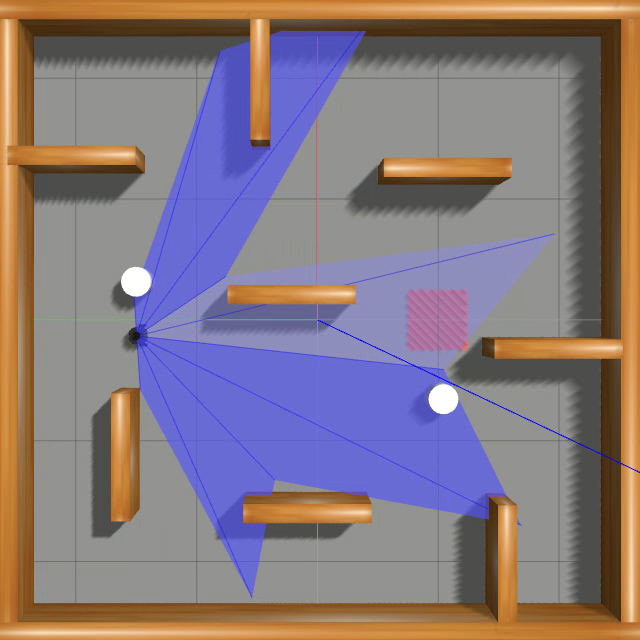
\includegraphics[width=\textwidth]{imagens/simulated_envs/sim_env3_sac/2.png}
        \end{subfigure}
        \hfill
        \begin{subfigure}[b]{0.24\textwidth}
            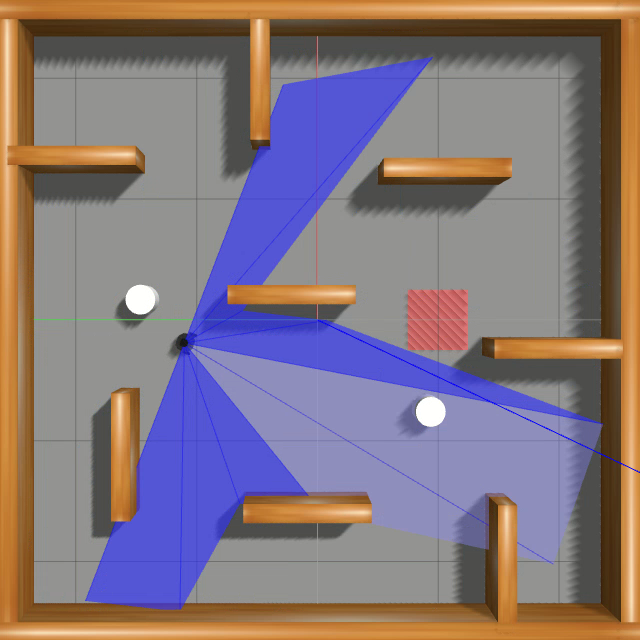
\includegraphics[width=\textwidth]{imagens/simulated_envs/sim_env3_sac/3.png}
        \end{subfigure}
        \hfill
        \begin{subfigure}[b]{0.24\textwidth}
            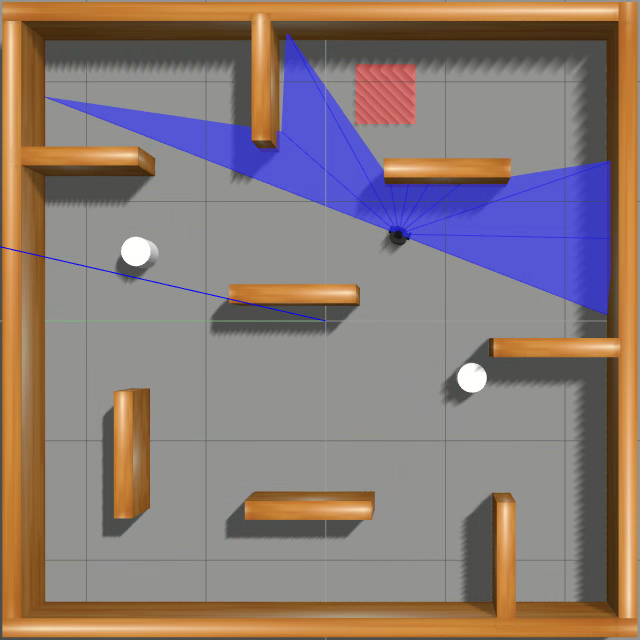
\includegraphics[width=\textwidth]{imagens/simulated_envs/sim_env3_ddpg/4.png}
        \end{subfigure}
        
        \begin{subfigure}[b]{0.24\textwidth}
            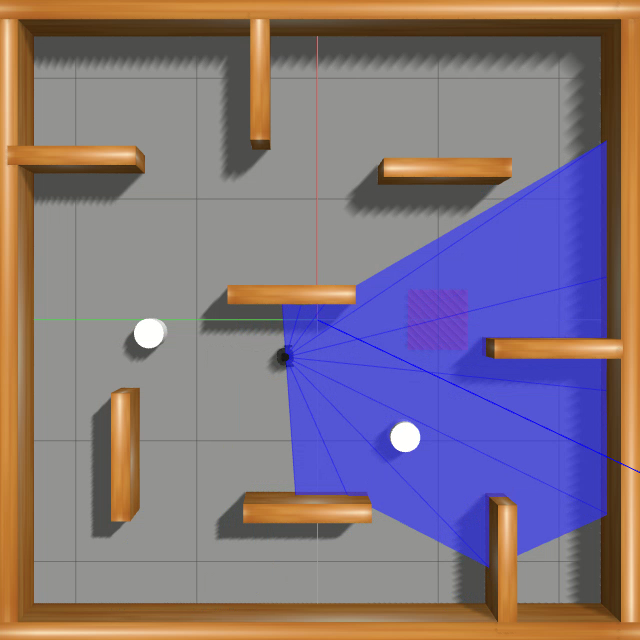
\includegraphics[width=\textwidth]{imagens/simulated_envs/sim_env3_sac/5.png}
        \end{subfigure}
        \hfill
        \begin{subfigure}[b]{0.24\textwidth}
            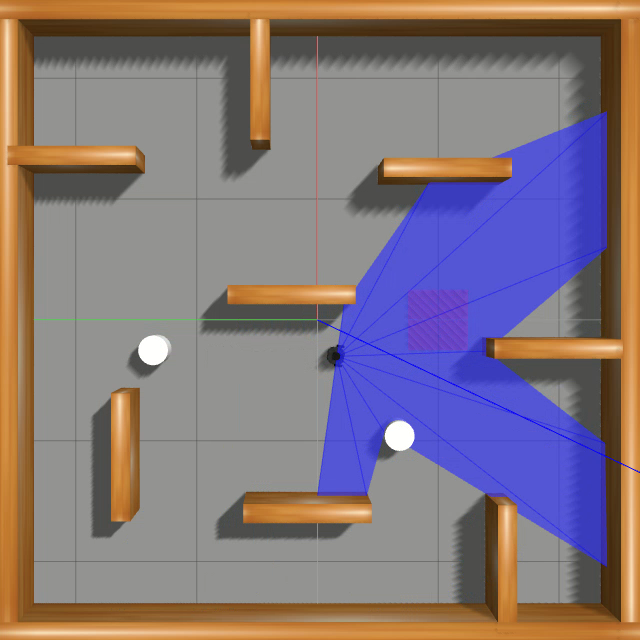
\includegraphics[width=\textwidth]{imagens/simulated_envs/sim_env3_sac/6.png}
        \end{subfigure}
        \hfill
        \begin{subfigure}[b]{0.24\textwidth}
            \includegraphics[width=\textwidth]{imagens/simulated_envs/sim_env3_sac/7.png}
        \end{subfigure}
        \hfill
        \begin{subfigure}[b]{0.24\textwidth}
            \includegraphics[width=\textwidth]{imagens/simulated_envs/sim_env3_sac/7.png}
        \end{subfigure}
        \caption{Rede SAC}
        \label{subfig:simulated_env3_sac}
    \end{subfigure}
    \label{fig:sim_env3}
    \end{center}
\small{Fonte: Autor}
\end{figure}

Os resultados da função de recompensa do último ambiente de treinamento é mostrado na Figura \ref{fig:stage_4}. 
Neste ambiente, por causa da alta complexidade, foi necessário um numero maior de episódios de treinamento.
Se comparado com as funções de recompensa anterior, da Figura \ref{fig:stage_1} e Figura \ref{fig:stage_4}, é possível notar uma recompensa média abaixo de dois mil para a rede DDPG da Figura \ref{subfig:ddpg_stage_4}.
Isso acontece pois para chegar ao alvo, que tem a maior recompensa possível em comparação com as outras recompensas, é necessário que o agente possa executar ações que geram menos pontos, contudo a rede DDPG ainda consegue chegar até o alvo. 
Já se for analisada a Figura \ref{subfig:sac_stage_4}, é visto que só nos primeiros episódios iniciais que ela apresenta um recompensa por episódio menor que dois mil, sem falar no menor tempo de treinos para ela superar a rede DDPG mesmo em relação ao treinamento do segundo ambiente que é mais simples que o terceiro ambiente de simulado.
Apesar disso, foi notado simulando o robô treinado algumas ações que causam o agente a colidir.
Muita dessas colisões foram devidas ao obstáculo dinâmico em movimento perto do alvo.
Isso resultou no agente fazer a decisão de que Turtlebot simulado poderia colidir ou tentar evitar o obstaculo móvel.
O comportamento ocorrido pode ter sido causado por causa do sistema de recompensa criado.
Em ordem de resolver essas ações, provavelmente, seria necessário criar uma função de recompensa que pudesse ignorar o erro para as redes treinadas.

\vspace{0.25cm} 
\begin{figure}[H]
\caption{Recompensas do terceiro ambiente simulado}
    \begin{center}
    \begin{subfigure}[b]{0.48\textwidth}
        \includegraphics[width=\textwidth]{imagens/simulated_envs/ddpg_stage_4.png}
        \caption{Rede DDPG}
        \label{subfig:ddpg_stage_4}
    \end{subfigure}
    ~
    \begin{subfigure}[b]{0.48\textwidth}
        \includegraphics[width=\textwidth]{imagens/simulated_envs/sac_stage_4.png}
        \caption{Rede SAC}
        \label{subfig:sac_stage_4}
    \end{subfigure}
    \end{center}
    \label{fig:stage_4}
\small{Fonte: Autor}
\end{figure}

%% escrever algo aqui. tipo "como notado nas recompensas da figura tal, figura tal e figural tal, a rede sac apresentou resultados melhores que a rede ddpg"
%%
%%
%%
%%
%%

\section{Experimentos com Turtlebot em Ambiente Real}

Depois do treinamento e validação de cada ambiente de simulação, foram utilizados dois ambientes reais, apresentados na Figura \ref{fig:real_environments}, para testar a rede DDPG e SAC no mundo real.
Com o alvo definido no primeiro no primeiro ambiente real, foram executadas a rede DDPG e SAC no Turtlebot3 versão Burger.
Nos gráficos, mostrados na Figura \ref{fig:real_env1}, é possível ver a trajetória feita pela rede DDPG e SAC  para chegar até o alvo.
O robô começa no ponto $(0,0)$ e faz uma trajetória para conseguir ir ao alvo.
É possível ver que ambas as redes, DDPG e SAC, conseguiram chegar ao alvo definido em um ambiente real.
A Figura \ref{fig:real_env1_frames} mostra por quadros de imagem a trajetória feita pelo robô para completar a tarefa.

\vspace{0.25cm} 
\begin{figure}[H]
\caption{Trajetória do Turtlebot3 no primeiro ambiente real}
    \begin{center}
    \begin{subfigure}[b]{0.48\textwidth}
        \includegraphics[width=\textwidth]{imagens/real_envs/real_env1_ddpg/graph.png}
        \caption{Rede DDPG}
        \label{subfig:ddpg_real_env1}
    \end{subfigure}
    ~
    \begin{subfigure}[b]{0.48\textwidth}
        \includegraphics[width=\textwidth]{imagens/real_envs/real_env1_sac/graph.png}
        \caption{Rede SAC}
        \label{subfig:sac_real_env1}
    \end{subfigure}
    \end{center}
    \label{fig:real_env1}
\small{Fonte: Autor}
\end{figure}

% ibagens
\vspace{0.25cm}
\begin{figure}[H]
\caption{Imagens sequência do experimento no Turtlebot3 no primeiro ambiente real}
    \begin{center}
    \begin{subfigure}[b]{0.60\textwidth}
        \begin{subfigure}[b]{0.24\textwidth}
            \includegraphics[width=\textwidth]{imagens/real_envs/real_env1_ddpg/1.png}
        \end{subfigure}
        \hfill
        \begin{subfigure}[b]{0.24\textwidth}
            \includegraphics[width=\textwidth]{imagens/real_envs/real_env1_ddpg/2.png}
        \end{subfigure}
        \hfill
        \begin{subfigure}[b]{0.24\textwidth}
            \includegraphics[width=\textwidth]{imagens/real_envs/real_env1_ddpg/3.png}
        \end{subfigure}
        \hfill
        \begin{subfigure}[b]{0.24\textwidth}
            \includegraphics[width=\textwidth]{imagens/real_envs/real_env1_ddpg/4.png}
        \end{subfigure}
        
        \begin{subfigure}[b]{0.24\textwidth}
            \includegraphics[width=\textwidth]{imagens/real_envs/real_env1_ddpg/5.png}
        \end{subfigure}
        \hfill
        \begin{subfigure}[b]{0.24\textwidth}
            \includegraphics[width=\textwidth]{imagens/real_envs/real_env1_ddpg/6.png}
        \end{subfigure}
        \hfill
        \begin{subfigure}[b]{0.24\textwidth}
            \includegraphics[width=\textwidth]{imagens/real_envs/real_env1_ddpg/7.png}
        \end{subfigure}
        \hfill
        \begin{subfigure}[b]{0.24\textwidth}
            \includegraphics[width=\textwidth]{imagens/real_envs/real_env1_ddpg/7.png}
        \end{subfigure}
        \caption{Rede DDPG}
        \label{subfig:real_env1_ddpg}
    \end{subfigure}
     %add desired spacing between images, e. g. ~, \quad, \qquad, \hfill etc. 
      %(or a blank line to force the subfigure onto a new line)
      
    \begin{subfigure}[b]{0.60\textwidth}
        \begin{subfigure}[b]{0.24\textwidth}
            \includegraphics[width=\textwidth]{imagens/real_envs/real_env1_sac/1.png}
        \end{subfigure}
        \hfill
        \begin{subfigure}[b]{0.24\textwidth}
            \includegraphics[width=\textwidth]{imagens/real_envs/real_env1_sac/2.png}
        \end{subfigure}
        \hfill
        \begin{subfigure}[b]{0.24\textwidth}
            \includegraphics[width=\textwidth]{imagens/real_envs/real_env1_sac/3.png}
        \end{subfigure}
        \hfill
        \begin{subfigure}[b]{0.24\textwidth}
            \includegraphics[width=\textwidth]{imagens/real_envs/real_env1_ddpg/4.png}
        \end{subfigure}
        
        \begin{subfigure}[b]{0.24\textwidth}
            \includegraphics[width=\textwidth]{imagens/real_envs/real_env1_sac/5.png}
        \end{subfigure}
        \hfill
        \begin{subfigure}[b]{0.24\textwidth}
            \includegraphics[width=\textwidth]{imagens/real_envs/real_env1_sac/6.png}
        \end{subfigure}
        \hfill
        \begin{subfigure}[b]{0.24\textwidth}
            \includegraphics[width=\textwidth]{imagens/real_envs/real_env1_sac/7.png}
        \end{subfigure}
        \hfill
        \begin{subfigure}[b]{0.24\textwidth}
            \includegraphics[width=\textwidth]{imagens/real_envs/real_env1_sac/7.png}
        \end{subfigure}
        \caption{Rede SAC}
        \label{subfig:real_env1_sac}
    \end{subfigure}
    \label{fig:real_env1_frames}
    \end{center}
\small{Fonte: Autor}
\end{figure}

Para o teste final das redes, foi usado o segundo ambiente real. Nos gráficos, mostrados na Figura \ref{fig:real_env2}, o robô começa no ponto $(0,0)$ e mesmo com obstáculos a rede DDPG e SAC são capazes de chegar ao alvo do ambiente.
Na Figura \ref{fig:real_env2_frames} é mostrado por quadros de imagem a trajetória feita pelo robô móvel para completar a tarefa.

\vspace{0.25cm} 
\begin{figure}[H]
\caption{Trajetória do Turtlebot3 no segundo ambiente real}
    \begin{center}
    \begin{subfigure}[b]{0.48\textwidth}
        \includegraphics[width=\textwidth]{imagens/real_envs/real_env2_ddpg/graph.png}
        \caption{Rede DDPG}
        \label{subfig:ddpg_real_env2}
    \end{subfigure}
    ~
    \begin{subfigure}[b]{0.48\textwidth}
        \includegraphics[width=\textwidth]{imagens/real_envs/real_env2_sac/graph.png}
        \caption{Rede SAC}
        \label{subfig:sac_real_env2}
    \end{subfigure}
    \end{center}
    \label{fig:real_env2}
\small{Fonte: Autor}
\end{figure}

% ibagens
\vspace{0.25cm}
\begin{figure}[H]
\caption{Imagens sequência do experimento no Turtlebot3 no segundo ambiente real}
    \begin{center}
    \begin{subfigure}[b]{0.60\textwidth}
        \begin{subfigure}[b]{0.24\textwidth}
            \includegraphics[width=\textwidth]{imagens/real_envs/real_env2_ddpg/1.png}
        \end{subfigure}
        \hfill
        \begin{subfigure}[b]{0.24\textwidth}
            \includegraphics[width=\textwidth]{imagens/real_envs/real_env2_ddpg/2.png}
        \end{subfigure}
        \hfill
        \begin{subfigure}[b]{0.24\textwidth}
            \includegraphics[width=\textwidth]{imagens/real_envs/real_env2_ddpg/3.png}
        \end{subfigure}
        \hfill
        \begin{subfigure}[b]{0.24\textwidth}
            \includegraphics[width=\textwidth]{imagens/real_envs/real_env2_ddpg/4.png}
        \end{subfigure}
        
        \begin{subfigure}[b]{0.24\textwidth}
            \includegraphics[width=\textwidth]{imagens/real_envs/real_env2_ddpg/5.png}
        \end{subfigure}
        \hfill
        \begin{subfigure}[b]{0.24\textwidth}
            \includegraphics[width=\textwidth]{imagens/real_envs/real_env2_ddpg/6.png}
        \end{subfigure}
        \hfill
        \begin{subfigure}[b]{0.24\textwidth}
            \includegraphics[width=\textwidth]{imagens/real_envs/real_env2_ddpg/7.png}
        \end{subfigure}
        \hfill
        \begin{subfigure}[b]{0.24\textwidth}
            \includegraphics[width=\textwidth]{imagens/real_envs/real_env2_ddpg/7.png}
        \end{subfigure}
        \caption{Rede DDPG}
        \label{subfig:real_env2_ddpg}
    \end{subfigure}
     %add desired spacing between images, e. g. ~, \quad, \qquad, \hfill etc. 
      %(or a blank line to force the subfigure onto a new line)
      
    \begin{subfigure}[b]{0.60\textwidth}
        \begin{subfigure}[b]{0.24\textwidth}
            \includegraphics[width=\textwidth]{imagens/real_envs/real_env2_sac/1.png}
        \end{subfigure}
        \hfill
        \begin{subfigure}[b]{0.24\textwidth}
            \includegraphics[width=\textwidth]{imagens/real_envs/real_env2_sac/2.png}
        \end{subfigure}
        \hfill
        \begin{subfigure}[b]{0.24\textwidth}
            \includegraphics[width=\textwidth]{imagens/real_envs/real_env2_sac/3.png}
        \end{subfigure}
        \hfill
        \begin{subfigure}[b]{0.24\textwidth}
            \includegraphics[width=\textwidth]{imagens/real_envs/real_env2_ddpg/4.png}
        \end{subfigure}
        
        \begin{subfigure}[b]{0.24\textwidth}
            \includegraphics[width=\textwidth]{imagens/real_envs/real_env2_sac/5.png}
        \end{subfigure}
        \hfill
        \begin{subfigure}[b]{0.24\textwidth}
            \includegraphics[width=\textwidth]{imagens/real_envs/real_env2_sac/6.png}
        \end{subfigure}
        \hfill
        \begin{subfigure}[b]{0.24\textwidth}
            \includegraphics[width=\textwidth]{imagens/real_envs/real_env2_sac/7.png}
        \end{subfigure}
        \hfill
        \begin{subfigure}[b]{0.24\textwidth}
            \includegraphics[width=\textwidth]{imagens/real_envs/real_env2_sac/7.png}
        \end{subfigure}
        \caption{Rede SAC}
        \label{subfig:real_env2_sac}
    \end{subfigure}
    \label{fig:real_env2_frames}
    \end{center}
\small{Fonte: Autor}
\end{figure}

O robô Turtlebot3 foi capaz de realizar ambas as tarefas dadas nos ambientes do mundo real.
Isso mostra o quão efetivo podem ser as redes DDPG e SAC, treinadas em ambientes de simulação, em completar tarefas complexas em ambientes físicos.